% !TeX root = ../index.tex

\section{Applikationsschicht}

Die Aufgaben der Anwendungsschicht sind es die von den Sensoren gesammelten Daten zu speichern und auf ihnen aufbauend die Aktoren zu steuern.
Zu diesem Zwecke ist eine Instanz der Low-Code/No-Code Plattform NodeRED auf einer \gls{vm} in der Computing-Infrastruktur der DHBW Mannheim installiert.
Die Plattform erlaubt es über eine einfache, grafische Benutzeroberfläche Programmabläufe zu gestalten und bietet viele vorgefertigte Integrationen zu Softwarelösungen welche im \gls{iot} beliebt sind.

Zum Beispiel MQTT und die Time-Series-Datenbank InfluxDB.
Letztere ist ebenfalls auf der \gls{vm} installiert und dient der Speicherung und Auswertung der Sensorwerte.

In der NodeRED-Umgebung sind die folgenden Anwendungsszenarien umgesetzt: Speicherung der Sensordaten, Steuerung der Pumpe, Steuerung der Markise und die Interaktion mit dem Nutzer über einen Bot für den Messenger-Dienst Telegram.
Das letzte Anwendungsszenario konnte allerdings im Rahmen des Labors nicht vollendet werden.

Die Logik zur Speicherung der Sensordaten ist simpel.
Je ein Programmablauf in NodeRED hört auf die topics für die verschiedenen Sensorwerte, formt die Daten leicht um und schreibt sie in die InfluxDB.
Die Steuerung von Pumpe und Markise sind allerdings komplizierter und werden daher im Folgenden nochmal im Detail beschrieben.

\subsection{Steuerung der Pumpe}

Das System soll selbstständig in regelmäßigen Abständen überprüfen, ob die Bodenfeuchtigkeit unter 25\% liegt.
Ist dies der Fall und falls für die nächsten 24 Stunden kein Niederschlag vorhergesagt ist, so soll die Pumpe aktiviert werden.

Die Pumpe soll für zwei Minuten laufen, um die Felder zu bewässern, und anschließend wieder deaktiviert werden.
Damit das Wasser Zeit zum Versickern hat, soll die Prüfschleife für fünf Minuten nach Aktivieren der Pumpe ausgesetzt werden.

\begin{figure}[h]
  \centering
  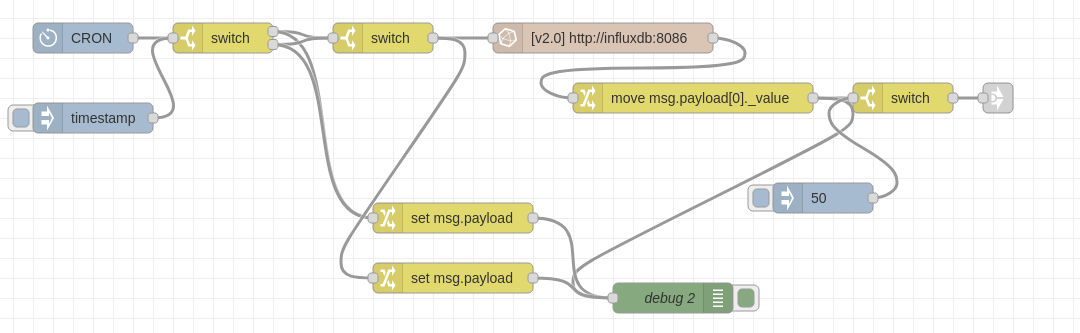
\includegraphics[width=\textwidth]{pump-activation.png}
  \caption{Überprüfungslogik für Pumpe in NodeRED}\label{fig:pump-activation}
\end{figure}

Abbildung \ref{fig:pump-activation} zeigt einen Screenshot der Überprüfungslogik für die Pumpe in NodeRED.
Das Programm wird jede Minute von dem CRON-Trigger gestartet und überprüft zunächst ob ein globales Flag gesetzt ist, welches die Überprüfung aussetzten würde.
Darauffolgend überprüft das Programm, ob für die nächsten 24 Stunden Niederschlag vorhergesagt ist.
Die Wetterdaten hierzu werden in einem Sub-Programm regelmäßig von der öffentlichen API des Deutschen Wetterdienstes geladen und in einer globalen Variable gespeichert.

Falls nicht, erfragt das Programm den durchschnittlichen Bodenfeuchtigkeitswert der letzten fünf Minuten von der InfluxDB.
Liegt dieser Wert unter 25\%, wird die Steuerungslogik für die Pumpe in einem Sub-Programm ausgeführt.
Dieses ist in Abbildung \ref{fig:pump-activation} dargestellt.

\begin{figure}[h]
  \centering
  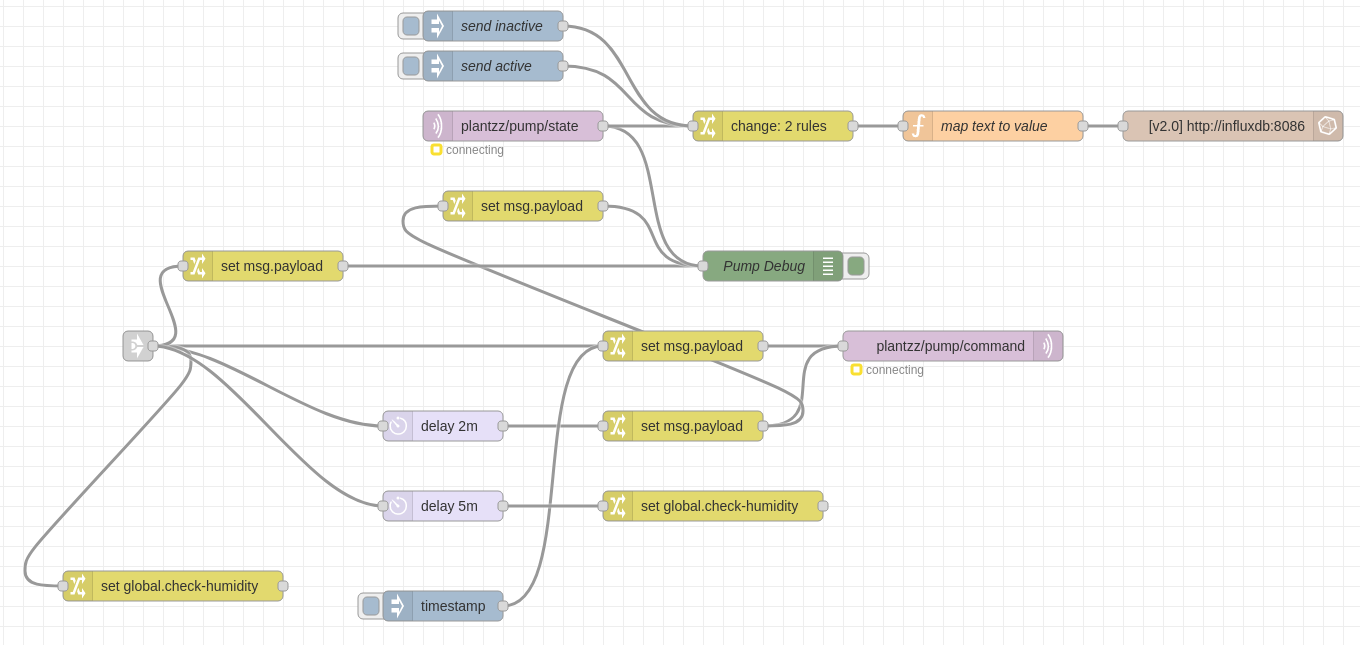
\includegraphics[width=\textwidth]{pump-control.png}
  \caption{Steuerungslogik für Pumpe in NodeRED}\label{fig:pump-activation}
\end{figure}

Beim Starten des Steuerungs-Programms wird unmittelbar eine Nachricht mit dem Aktivierungskommando an das MQTT-Topic der Pumpensteuerung versendet.
Zudem wird das globale Flag gesetzt, welches die die Überprüfungslogik deaktiviert.
Nach einer Verzögerung von zwei Minuten, wird das Deaktivierungskommando versendet und nach fünf Minuten wird das Flag zur Deaktivierung der Überprüfungslogik wieder zurückgesetzt.

\subsection{Steuerung der Markise}
Das System soll fähig sein selbstständig zu überprüfen ob eine Beschattung durch eine Markise momentan benötigt wird. Um  das Ein- und Ausfahren dieser Markise automatisch zu steuern werden einige Umwelteinflüsse überprüft. Die Markise ist im Allgemeinen von der Helligkeit abhängig. Weitere Faktoren, die ebenfalls zur Steuerung der Markise mit einbezogen werden sind außerdem die Windgeschwindigkeit, die aus Wetterdaten entnommen wird, und die Umgebungstemperatur. 
Die folgende Abbildung \ref{fig:canvas-activation} zeigt den Ablauf der Überprüfung. Das Programm startet wie auch bei der Pumpensteuerung mit einem CRON-Trigger einmal pro Minute.

\begin{figure}[h]
  \centering
  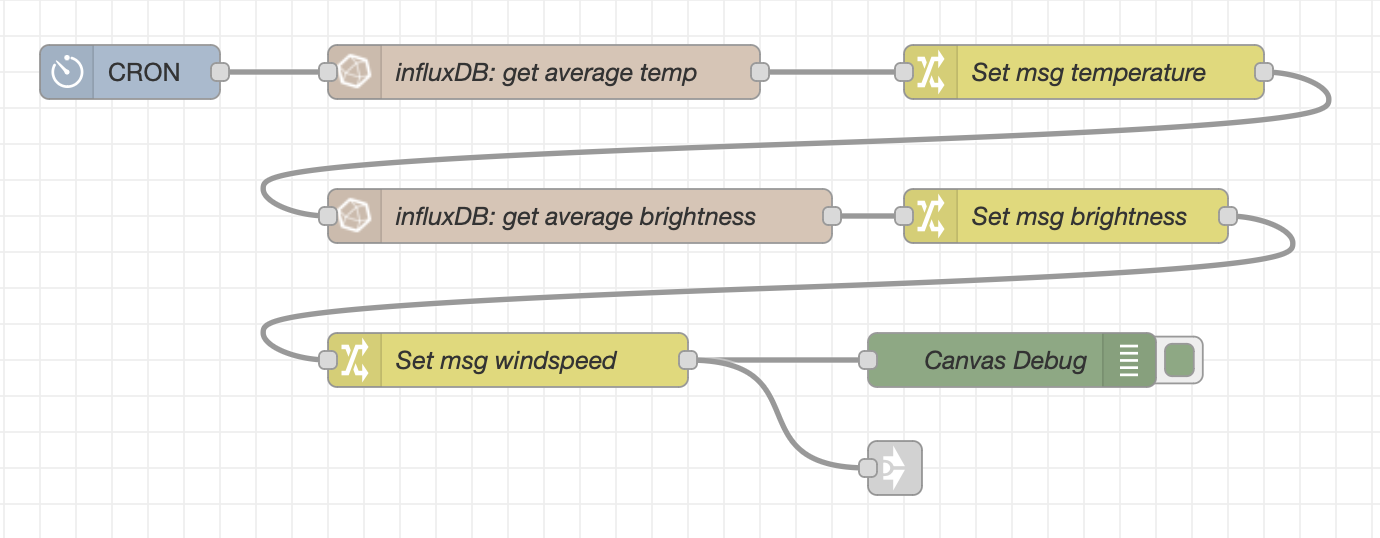
\includegraphics[width=\textwidth]{canvas-activation.png}
  \caption{Überprüfungslogik für die Markise in NodeRED}\label{fig:canvas-activation}
\end{figure}

Damit die Markise ausfährt werden hintereinander die drei Kriterien überprüft. Wenn der Durschnitt der Umgebungstemperatur der letzten 5 Minuten über 20° Celsius liegt ist der erste Check bestanden. Diese Grenze wurde eingeführt, da eine Beschattung im Sommer beziehungsweise bei hohen Temperaturen hilft damit die Pflanzen nicht austrocken, bei kälteren Temperaturen würde eine Beschattung wertvolle Sonnenstrahlen von den Pflanzen abhalten.
Die zweite Überprüfung betrifft die Helligkeit, für welche ebenfalls der Durschnittswert der letzen 5 Minuten ausschlaggebend ist. Wenn dieser Wert über 75\% liegt ist ein weiterer Kontrollpunkt überschritten.
Der letzte Punkt, der noch überprüft wird, dient der Unversertheit der Markise. Die Markise darf nur ausfahren wenn die Windgeschwindigkeit von 14 m/s nicht überschritten ist.

\begin{figure}[h]
  \centering
  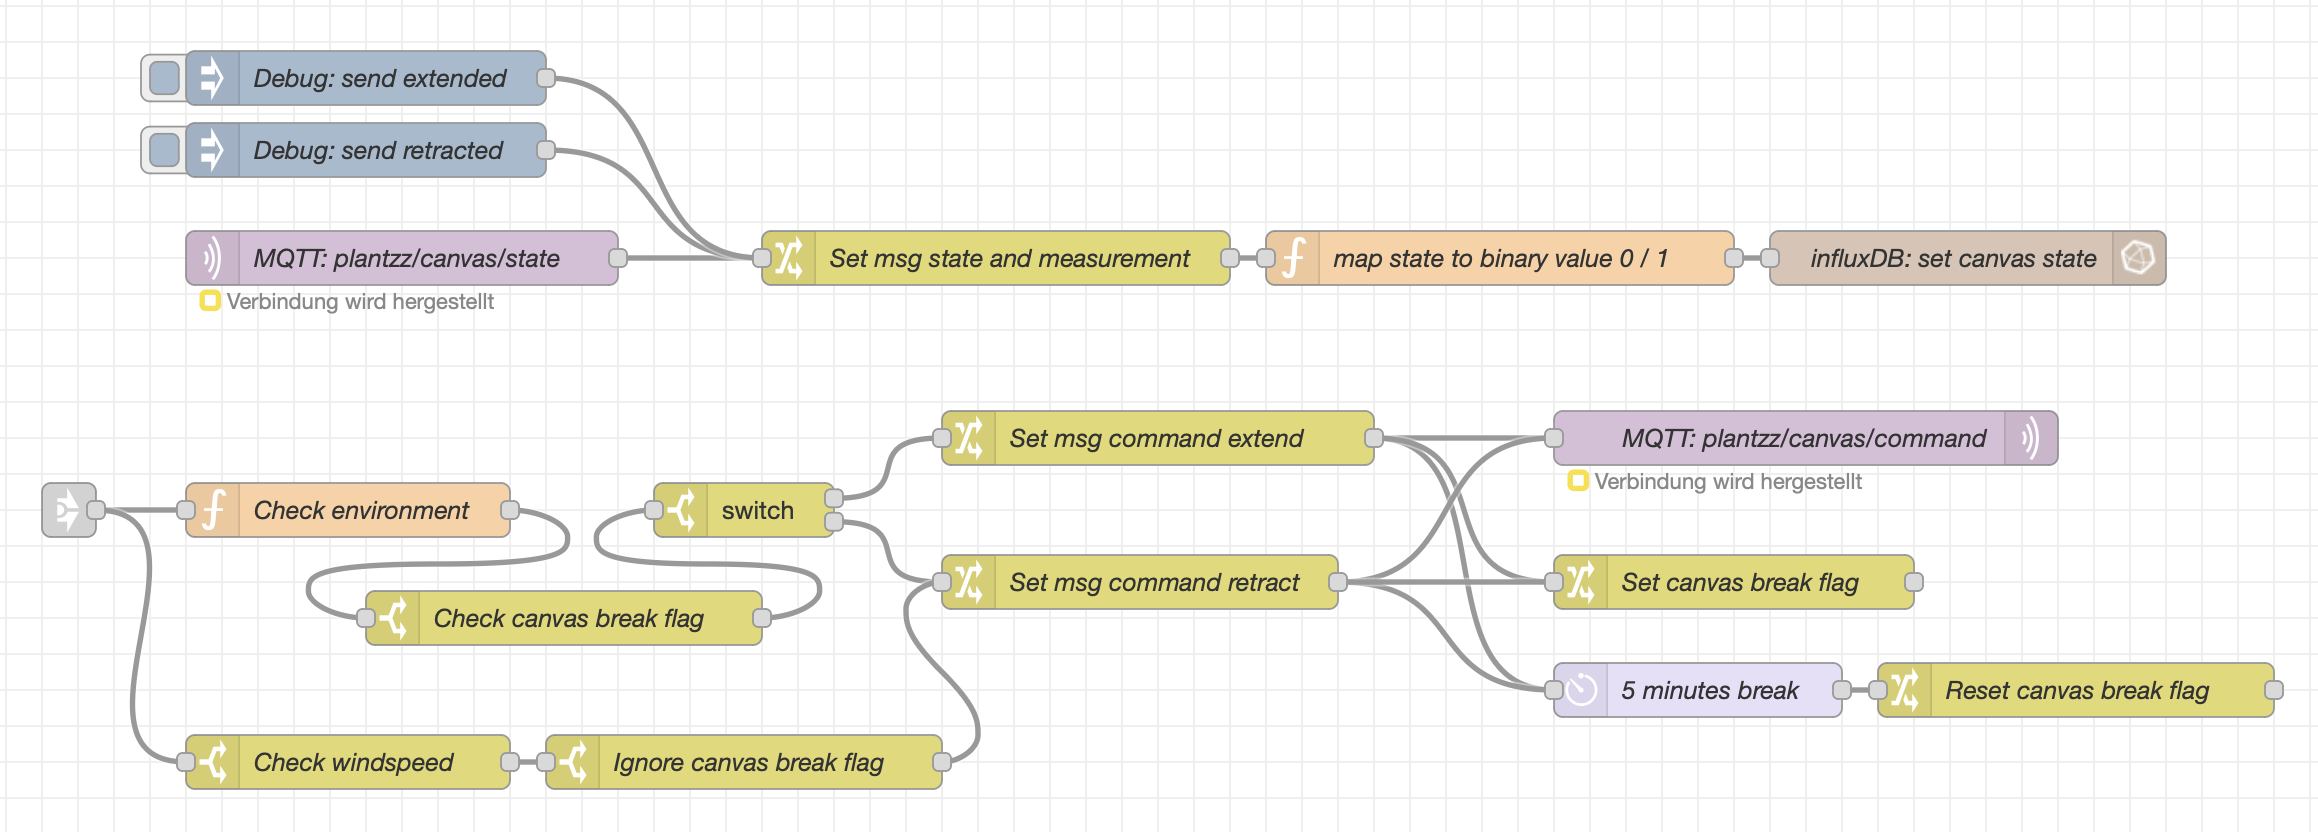
\includegraphics[width=\textwidth]{canvas-control.png}
  \caption{Steuerungslogik für Pumpe in NodeRED}\label{fig:canvas-activation}
\end{figure}

Beim Übergang zur Markisensteuerung werden in "function 1" zunächst die bereits beschriebenen checks durchgeführt wofür zuvor die Information gespeichert und verarbeitet wurden. Wenn die Freigabe zum Überprüfen der Helligkeit erteilt ist, wird danach abhängig vom Ergebnis der drei Überprüfung entweder die Markise ein oder ausgefahren. Parallel dazu wird die Windgeschwindigkeit als einzelnes Kriterium auch wenn die Freigabe für die Helligkeitsüberprüfung nicht erteilt ist um die Markise bei Überschreiten des Grenzwerts einfahren zu lassen.
Sobald der Befehl zum Ein- oder Ausfahren der Markise erteilt wurde, wird gleichzeitig die Freigabe zum erneuten Überprüfen der Helligkeit für 5 Minuten deaktiviert um ein andauerndes Ein- und Ausfahren bei sich leicht ändernden Bedingungen im Grenzbereich zu verhindern.